\section{Output Checking Protocol} \label{sec:output}

Most server programs are multithreaded and they may run into nondeterminism 
(\eg, concurrency errors~\cite{lu:concurrency-bugs}), which may cause replicas 
to diverge. \xxx provides a fast output checking protocol for a practical 
purpose: improving \xxx users' assurance on whether replicas run in sync. If 
diverged replicas are detected, users can restore the them 
(\S\ref{sec:checkpoint}).

% TBD. Motivation of this approach. Make replicas follow consistent execution 
% states. Recover from bugs that diverge executions. 
% This section presents \xxx's output checking protocol for detecting and 
% recovering from replicas' execution divergence. This section first introduces 
% how \xxx computes and compares network outputs among replicas 
% (\S\ref{sec:output-workflow}), and then introduces its checkpoint and rollback 
% mechanism to deal with divergence (\S\ref{sec:checkpoint}).
% 
% \subsection{Checking Network Outputs} \label{sec:output-workflow}

% Main issue. Output timings are pretty miscellaneous.
A main technical challenge for comparing outputs across replicas is that 
network outputs and their physical timings are miscellaneous. For example, when 
we ran \redis simply on pure SET workloads, we found that different replicas 
reply the numbers of ``OK" replies for SET operations randomly: one replica may 
send four of them in one \send call, while another replica may only send one of 
them in each \send call. Therefore, comparing outputs on each \send call among 
replicas may not only yield wrong results, but may slow down server programs 
among replicas.

% Two variables. Tckpt (checkpoint periods) and Tcmp (comparison periods).
To tackle this challenge, \xxx presents a bucket-based hash computation 
mechanism. When a server calls a \send call, \xxx puts the sent bytes into a 
local, per-connection bucket with 1.5KB (MTU size). Whenever a bucket 
is full, \xxx computes a new CRC64 hash on a union of the current hash and this 
bucket. Such a hash computation mechanism encodes accumulated network outputs. 
Then, for every \thashcomp (by default, 10K in \xxx) local hash values 
are generated, \xxx invokes the output checking protocol once to check this 
hash across replicas. Because this protocol is invoked rarely, it did not incur 
observable performance lost in our evaluation.

% The index of this hash in the generated sequence is consistent across 
% replicas because each replica runs the same mechanism to generate the hash 
% sequence.

% TBD. Briefly describe why using our input coordination protocol for output 
% checking is good. Simply the whole system, reliable (tolerate packet 
% lossses and consistency, thanks to paxos), fast, already have ACK mechanisms.

% Leverage the input protocol to carry the hash of outputs. Occasionally.
To compare a hash across replicas, \xxx's output checking protocol runs the 
same as the input coordination protocol (\S\ref{sec:normal}) except that the 
follower thread on each backup replica carries this hash value in the \v{reply} 
written back into the leader's corresponding log entry.

% To make an effort to 
% collect more remote hash values, \xxx waits for \twait (by default, 20 \us) 
% and then starts to detect divergence on hash values.

% This output protocol starts by letting a leader thread invoke a consensue 
% request on this hash comparison for its own client connection. The leader also 
% writes its own hash value in the \v{ack} array with its own replica ID. Then, 
% follower threads on backup replicas carry their local hash values in the \v{ack} 
% array according to the connection ID \v{conn\_vs}. Once a quorum of \v{ack} 
% is ready, the leader simply detects divergence with the hash values in its 
% local \v{ack} array. Note that at this moment, some replicas may not send back 
% their reply yet because only a quorum is reached. To make an effort to collect 
% a complete hash values, \xxx waits for \twait (by default, 20 \us) and then 
% starts to detect divergence on hash values.

% Figure~\ref{fig:divergence} shows the workflow on how the leader checks 
% present replies and handles divergence, which includes four shaded cases: 
% (1) all hashes are the same; (2) leader's hash equals a majority of replicas, 
% but minor replicas' hashes diverge; (3) leader's hash diverges from a majority 
% of replicas'; and (4) no majority has the same hash value. The first three 
% cases should be the normal case unless a program tends to frequently compute 
% outputs on random functions (\eg, a scientific simulator).
% 
% Currently \xxx has not incorporated an input re-planing approach (\eg, 
% Eve~\cite{eve:osdi12} sequentially re-executes requests after detecting a 
% execution divergence) because we found that re-execution already empirically
% avoided divergence. Previous work~\cite{lu:concurrency-bugs,pres:sosp09} 
% also confirmed that it was extremely unlikely to trigger a concurrency bug 
% twice in two consecutive executions.

% Even so, we can 
% leverage prior approaches to hook these 
% random functions~\cite{paxos:practical,eve:osdi12} and make them generate same 
% return values among replicas.

% Once the leader decides to roll back a diverged replica (including itself), it 
% invokes a local guard process (\S\ref{sec:overview}) that handles 
% checkpointing and rolling back the local server program. If a remote replica 
% needs to be rolled back, the local guard forwards the roll back request to the 
% guard in that remote replica.
% 
% We explicitly design this output checking protocol to be fast with two 
% considrations: (1) because the hash comparison consensus happens occasionally 
% (every \thashcomp hash generations), the performance penalty on this output 
% consensus is negligible; and (2) all or most replicas' hash values are 
% the same in normal case. Two parameters, \thashcomp and \twait, may be 
% sensitive to \xxx's performance. We did an evaluation on diverse server 
% programs and found that these default values are reasonable, general settings to 
% these programs (\S\ref{sec:sensitivity}).

% When divergence is detected, spawn the mechanism, show workflow.

% Strawmen approach? Necessary?
% 
% \begin{figure}[t]
% \centering
% \vspace{-.10in}
% 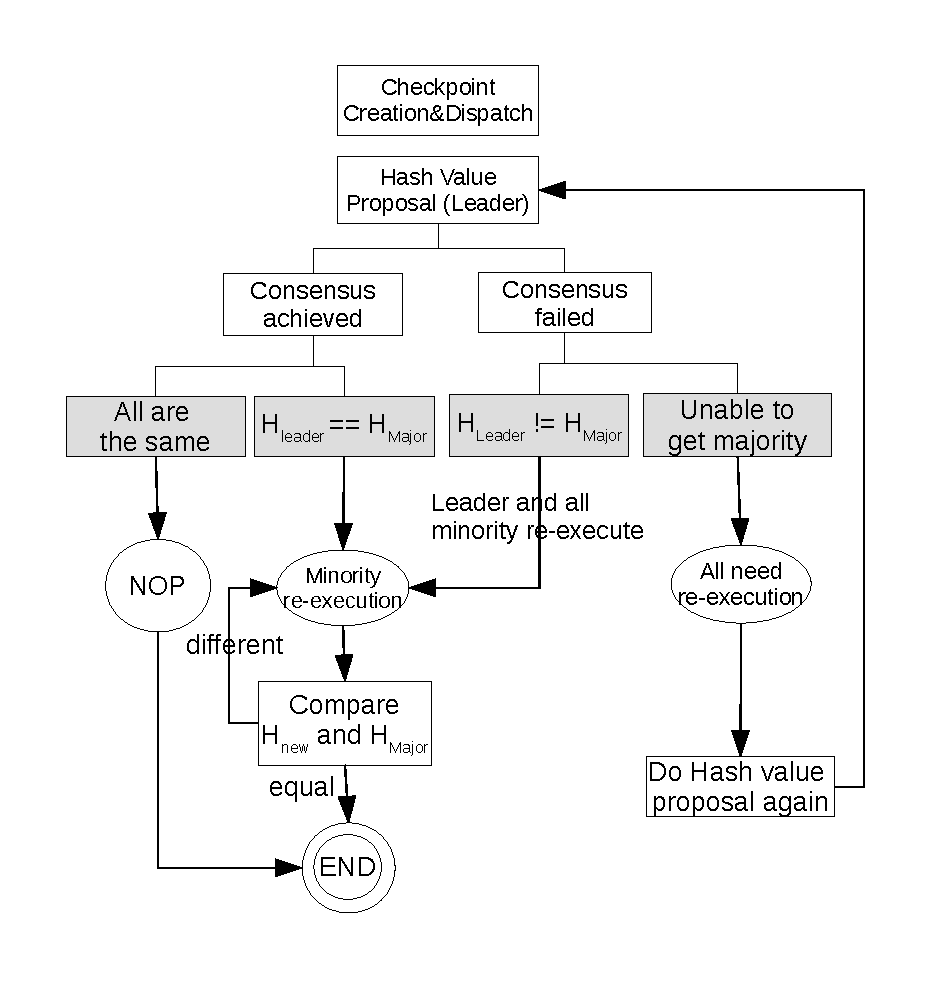
\includegraphics[width=.5\textwidth]{figures/output-divergence}
% \vspace{-.50in}
% \caption{{\em Workflow to Handle Network Output Divergence.}} 
% \label{fig:divergence}
% \vspace{-.20in}
% \end{figure}


% Suppose the 
% viewstamp associated with the 
% % previous checkpoint is $vs_{ckpt}$, and the viewstamp of the last matching 
% hash 
% % comparison log entry is $vs_{match}$, \xxx ensures that $vs_{ckpt}$ 
% % is smaller than $vs_{match}$ so that this checkpoint is not diverged.

% After checkpointing process state, \xxx uses CRIU to stop this process and then 
% zip files in the process's current working directory recursively, including the 
% socket call stable storage (\S\ref{sec:input}). In our evaluation, 
% zipping current working directory was sufficient to carry all files used 
% by the evaluated programs.

% To avoid a server 
% to modify files missed by \xxx, we only assign a server process write 
% permissions to its current working directory and the ``/tmp" directory (files in 
% ``/tmp" directory often do not matter). \xxx's file system checkpoint avoids the 
% need of comparing program outputs to the file system.

% Closing RDMA sockets before checkpoint because CRIU does not support such 
% special memory.



% Orthogonal to the \paxos protocol, just feel like some replicas restart 
% themselves. Paxos can handle this.

% Sound. As long as local machines have a checkpoint with a viewstamp before 
% the last matched output check.

% Closing RDMA sockets before checkpoint because CRIU does not support such 
% special memory.


% \subsection{Efficiency and Reliability} \label{sec:output-discuss}
% % Efficient. Occasionally check hash. 
% 
% % Sound. If Tckpt is longer than Tcomp.


